\documentclass[10pt,twocolumn]{article}

\usepackage[margin=0.72in]{geometry}
\usepackage{graphicx}
\usepackage{booktabs}
\usepackage{array}
\usepackage{multirow}
\usepackage{amsmath}
\usepackage{amssymb}
\usepackage{xurl}
\usepackage[numbers,sort&compress]{natbib}
\usepackage[hidelinks]{hyperref}
\usepackage{caption}
\usepackage{subcaption}
\captionsetup{font=small}
\captionsetup[sub]{font=small}
\usepackage{float}
\usepackage{balance}

\graphicspath{{../plots/report/}}
\setlength{\columnsep}{0.22in}
\setlength{\parskip}{0.15em}
\setlength{\parindent}{0.8em}

\title{\vspace{-0.4in}Predicting Grocery Reorders: A Controlled Error Analysis of Classical Machine Learning Models}
\author{}
\date{}

\begin{document}
\maketitle

\begin{abstract}
This project studies grocery reorder prediction using the Instacart Online Grocery Shopping Dataset. Rather than optimizing for leaderboard performance, we compare logistic regression, random forest, AdaBoost, and XGBoost under a shared, leakage-controlled feature set. The task is framed as binary classification over historical user--product pairs. Random forest performs best as a row-level classifier (F1: 0.5686), while logistic regression achieves the highest per-order F1 (0.2479) because it predicts systematically larger baskets. This metric-dependent reversal, combined with our behavioral error taxonomy, demonstrates that grocery recommender models must be evaluated not only by classification accuracy, but also by basket-size dynamics and the operational cost of false alarms versus missed staples.
\end{abstract}

\section{Introduction}

Online grocery reorder prediction is a next-basket recommendation problem: the system must decide which previously purchased products are likely to be bought again in the next order. Accurate next-basket prediction has direct commercial value: surfacing the right staple goods reduces friction in cart construction, raises average order value, and supports retention by removing the need for repeat customers to re-search for products they buy on a regular cadence. Rule-based recency heuristics --- such as ``recommend everything in the user's last order'' --- capture a meaningful slice of this signal but miss the user~$\times$~product~$\times$~time interactions that determine whether a particular staple actually returns this week. Machine learning is helpful precisely because those interactions are heterogeneous across users and product categories.

The Instacart dataset contains anonymized order histories for more than 200,000 users and over three million orders \citep{instacart2017dataset,kaggle2017instacart}. This report follows the project objective: compare model classes and analyze where they succeed and fail, rather than chase leaderboard performance. In an operational recommender, the right operating point depends on whether false positives (over-suggesting) or false negatives (missing a staple) are more costly, so the comparison emphasizes \emph{types} of errors made by each model class rather than a single headline F1 number. This distinction matters operationally: a model can improve row-level precision while worsening basket-level utility, or improve basket-level recall only by aggressively over-recommending products.

The prediction unit is a historical $(\text{user}, \text{product})$ pair. A row is positive if the user reordered that product in the target order. This denominator is important: the positive rate in our controlled final evaluation is 12.5\%, so accuracy alone is not meaningful. We therefore emphasize F1, PR-AUC, and basket-level analysis.

Our specific contributions are: (1) a leakage-controlled, shared-feature protocol that allows the four-way model comparison to cleanly attribute performance differences to the algorithm class; (2) dual-metric reporting (row-level vs.\ per-order F1) that surfaces a metric-dependent reversal in model rankings; and (3) a behavioral error taxonomy and disagreement-overlap analysis mapping where each model class fails differently.

\section{Related Work}

Public solutions to the Instacart Market Basket Analysis competition \citep{kaggle2017instacart} establish both the dominant feature design and the dominant model class for this task. \citet{onodera2017instacart} (2nd place) introduce the four-group feature taxonomy --- user-level, product-level, user~$\times$~product, and target-order datetime --- and show that direct, recency-windowed user~$\times$~product aggregations dominate his importance ranking, with the top features computed only over each user's most recent five orders. \citet{vasquez2017instacart} (3rd place) reaches comparable performance with a similar set of direct aggregations supplemented with deep learned product embeddings.

Public reimplementations confirm this feature-driven paradigm: \citet{olsonswanson2018instacart}, \citet{yu2017instacart}, and \citet{syntheticjohn2019instacart} report F1 progressions from 0.32 to 0.44 driven almost entirely by recency predictors with only minor gains from hyperparameter tuning, while \citet{rich2017instacart} and \citet{bhat2022instacart} confirm that expanding direct aggregations dominates architectural choice.

This work differs from prior public solutions on Instacart in three ways. First, the goal is not leaderboard optimization but a controlled comparison: all four supervised model classes are restricted to the same shared, leakage-controlled feature set (37 features after a logical pre-filter of 44 candidates), so performance differences are attributable to the learning algorithm rather than to feature differences. Second, instead of adding learned product embeddings \citep{vasquez2017instacart} or expanding to 76+ feature columns \citep{bhat2022instacart}, we hold the feature space fixed and pair the comparison with statistical tests (McNemar, DeLong, user-bootstrap) calibrated to the next-basket evaluation. Third, the analysis is organized around \emph{error modes} --- subgroup-level performance (cold-start, none-users, single-purchase pairs, high-variance aisles) and a behavioral error taxonomy (stockpile, broken streak, basket-size inflation, none-collapse) --- rather than around a single F1 number. The result is a comparison that surfaces \emph{which kinds of mistakes} each algorithm tends to make, not just which algorithm wins on average.

\section{Data and Problem Setup}
\label{sec:data}

The Instacart Online Grocery Shopping Dataset 2017 \citep{instacart2017dataset} comprises five tables (orders, prior order products, train order products, products, and aisle/department metadata) covering approximately 206{,}000 users, 3.4 million orders, and 50{,}000 products. The original Kaggle test labels are private, so the official Kaggle train users are repurposed as the fully labeled population. A custom 80/20 user-level split is used so that all candidate products for a given user remain entirely in either train or test, stratified by user-activity tier (low, medium, high prior-order count) so that all three activity strata are proportionally represented in train and test. This avoids leaking user-level behavior through features such as preferred order time, total prior orders, and prior reorder ratio, and ensures that the cold-start vs.\ power-user contrast in \S\ref{sec:strat} is interpreted as a generalization gap rather than a sampling artifact.

The binary classification problem in this work operates over historical $(\text{user}, \text{product})$ pairs, not over individual products in a basket. This denominator distinction is important. The often-quoted ``59\% reorder rate'' from Instacart refers to the share of \emph{items in a basket} that are reorders, not to the positive class rate of the prediction task. Over the candidate-pair table for the official Kaggle train users, the positive rate is 9.78\% (828{,}824 positives out of 8{,}474{,}661 pairs). For final controlled evaluation each model was evaluated on the same 75{,}000 held-out candidate rows from 6{,}484 users, giving a controlled-sample positive rate of 12.5\%. Concretely, the sample comprises the first 75{,}000 candidate rows of the held-out test split in its on-disk user-grouped order, which encompasses every candidate $(\text{user},\text{product})$ pair for the 6{,}484 contiguous test users that fit under the row cap; this preserves per-user basket integrity, so per-order F1 is well-defined for every user in the sample. Because the held-out users were already randomly assigned within the stratified user-level split before the parquet was written, this contiguous user-grouped slice preserves full user baskets without intentionally selecting users by outcome or activity. Because both rates are far from balanced, accuracy is not informative here; F1, PR-AUC, and basket-level analysis are reported instead. The average actual reordered basket size is 1.45 candidate products per user, while predicted basket size varies strongly by model.

\begin{figure}[htbp]
\centering
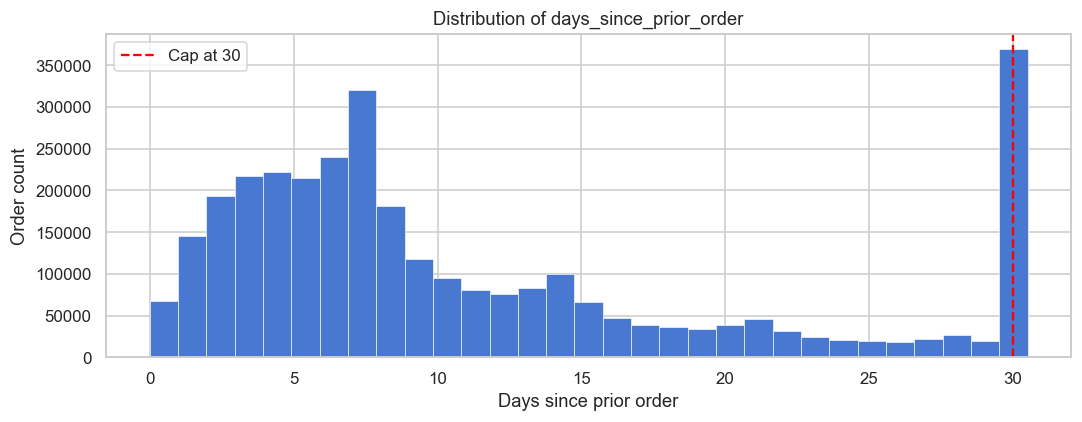
\includegraphics[width=\columnwidth]{eda_days_since_prior.png}\\
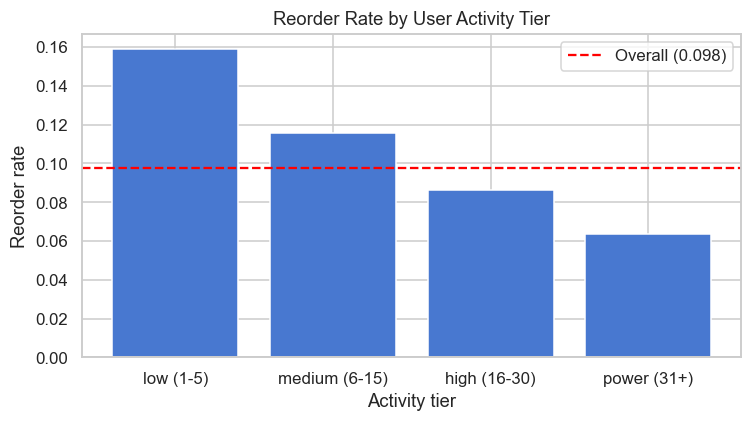
\includegraphics[width=0.85\columnwidth]{eda_reorder_by_activity.png}
\caption{Exploratory data analysis highlights. \textbf{Top:} the days-since-prior-order distribution exhibits an artificial spike at 30 (11.5\% of orders) due to Instacart's recording cap, motivating careful handling of recency features. \textbf{Bottom:} the candidate-pair positive rate decreases monotonically with user activity (0.16 for low-activity users, 0.06 for power users), because power users have a much larger denominator of historical products that could appear in the next basket; this directly motivates the cold-start vs.\ power-user contrast in the \S\ref{sec:strat} stratified analysis.}
\label{fig:eda}
\end{figure}

\section{Feature Engineering and Selection}

The feature set follows a shared-input design. All models receive the same engineered predictors before model-specific mechanical preprocessing. This choice isolates model-class effects: differences in performance and feature importance are attributable to the learning algorithm rather than to different input variables.

The candidate feature set was assembled from 44 predictors documented in prior public Instacart solutions and reduced to 37 through a logical pre-filter that removes deterministic redundancies (e.g., features that are exact arithmetic transformations of others; removed examples include \texttt{up\_purchase\_ratio\_n5}, \texttt{dow\_match\_user\_pref}, and \texttt{hour\_diff\_from\_user\_pref}). The 37 surviving features are organized into the four groups established by \citet{onodera2017instacart}: \textbf{user-level} features describing each user's general ordering cadence and preferences (e.g., total orders, average basket size, preferred day of week); \textbf{product-level} features describing each product's global popularity and reorder dynamics (e.g., total purchases, reorder ratio, average cart position); \textbf{user~$\times$~product} features describing the dyadic interaction history, including recency-windowed variants over the user's most recent five orders (purchase counts, orders/days since last purchase, streaks, ratios after first purchase); and \textbf{target-order datetime} features describing when the candidate basket is being placed (day of week, hour, days since prior order, user~$\times$~product day-of-week purchase counts). The recency-windowed user~$\times$~product features are retained because \citet{onodera2017instacart} reports them as the strongest predictors in his solution.

Feature selection proceeds in two stages. First, a logical pre-filter removes deterministic redundancies. Second, correlation and Variance Inflation Factor (VIF $> 5$) diagnostics are computed on training data only to guard against multicollinearity, especially for logistic regression coefficient stability \citep{belsley1980regression}. Categorical aisle and department identifiers are encoded differently by model class: tree models receive ordinal encodings, while logistic regression uses Laplace-smoothed target encoding for high-cardinality categoricals following \citet{micci2001target}, with the smoothing prior set to the global positive rate. The encoder is fit strictly within each cross-validation fold to prevent label leakage. Missing-value handling also differs by model class: XGBoost relies on its built-in default-direction NaN handling, whereas random forest, AdaBoost, and the numeric pipeline of logistic regression use median imputation fit on training rows only. This isolates model-class effects from imputation artifacts.

Leakage prevention is enforced programmatically: dedicated validators check (i) zero user overlap between splits, (ii) row preservation across feature merges, (iii) train-only scope of correlation and VIF diagnostics, (iv) target-encoding fit restricted to in-fold rows, and (v) absence of dropped pre-filter features in the final feature list. These checks run as part of the pipeline rather than as one-off scripts.

\section{Models and Training}

The comparison establishes a non-ML baseline and four classical supervised models, chosen so that each occupies a distinct point in the bias/variance and inductive-bias space rather than a different feature space. The \textbf{last-basket} baseline predicts exactly the products from the user's most recent prior order; it encodes the strict recency heuristic that next-basket recommendation systems must beat to justify any modeling at all, and is notoriously hard to outperform in this setting \citep{olsonswanson2018instacart}. \textbf{Logistic regression} provides a linear, additive decision-boundary reference model: with all four models on the same shared 37-feature space, any performance gap between logistic regression and the tree ensembles is attributable to non-linearity rather than to feature differences. \textbf{Random forest} represents bagging plus feature subsampling for variance reduction over decorrelated deep trees \citep{breiman2001random}. \textbf{AdaBoost} represents sequential reweighting boosting over shallow decision trees (depth 3), which contrasts deliberately with random forest's parallel deep-tree variance reduction \citep{freund1997adaboost}. \textbf{XGBoost} represents regularized gradient-boosted trees and is included because it has been the dominant model class on this dataset in prior public solutions \citep{chen2016xgboost,onodera2017instacart,syntheticjohn2019instacart}.

Logistic regression, random forest, and AdaBoost were trained with scikit-learn \citep{pedregosa2011sklearn}; XGBoost used the reference \texttt{xgboost} library \citep{chen2016xgboost}. Hyperparameter tuning used full grid search over the regularization strength $C$ for logistic regression, randomized search over depth, leaf-count, and subsampling parameters for random forest and AdaBoost \citep{bergstra2012random}, and Optuna-based Bayesian optimization \citep{akiba2019optuna} for XGBoost. All searches utilized 5-fold user-grouped cross-validation to keep all of a user's candidate rows in the same fold, preventing the user-level leakage described in \S\ref{sec:data}. Final classification thresholds are selected from validation F1 sweeps and then fixed prior to any held-out test evaluation.

\section{Evaluation Metrics}

Two F1 conventions are reported. Row-level F1 is computed globally across all candidate rows. Per-order F1 is computed per user basket and then averaged across users. Per-order F1 is defined as $0$ for any user with no true positives, including users for whom both the true basket and the predicted basket are empty; consequently none-users contribute zero to the per-order F1 average regardless of model behavior. The latter matches the next-basket framing and Kaggle-style evaluation more closely, while the former reveals row-wise discrimination quality across the candidate table. Per-order F1 is closer in spirit to the Kaggle evaluation than row-level F1, though it is not strictly leaderboard-comparable due to our controlled 75{,}000-row sample and shared-feature protocol; published per-order F1 scores in this setting typically range from 0.40 to 0.44 \citep{syntheticjohn2019instacart, olsonswanson2018instacart}.

Supplementary metrics are precision, recall, ROC-AUC, PR-AUC, miss rate, false-alarm rate, basket-size error, and error-overlap measures. For statistical testing, McNemar's test compares paired row-level prediction correctness \citep{mcnemar1947}, user-bootstrap confidence intervals compare per-order F1 differences, and DeLong's test compares paired ROC-AUC values \citep{delong1988}. Because the test set is large, practical effect sizes are interpreted alongside significance.

\section{Results}

\begin{table*}[t]
\centering
\caption{Final controlled model metrics. Row F1 is computed globally over candidate rows; per-order F1 is computed by user first and then averaged. Train (s) is total fit + inference time on the controlled-sample run.}
\label{tab:metrics}
\scriptsize
\begin{tabular}{lrrrrrrrrr}
\toprule
Model & Threshold & Precision & Recall & Row F1 & Per-order F1 & ROC-AUC & PR-AUC & Avg. Basket & Train (s) \\
\midrule
Random Forest & 0.43 & 0.4970 & 0.6642 & \textbf{0.5686} & 0.2425 & \textbf{0.9073} & 0.5845 & 1.93 & 52.0 \\
AdaBoost & 0.45 & 0.4816 & 0.6774 & 0.5630 & 0.2414 & 0.9020 & 0.5738 & 2.03 & 282.4 \\
XGBoost & 0.47 & 0.4768 & 0.6746 & 0.5587 & 0.2390 & 0.9046 & \textbf{0.5854} & 2.05 & 47.9 \\
Logistic Regression & 0.50 & 0.3132 & \textbf{0.7658} & 0.4446 & \textbf{0.2479} & 0.8429 & 0.4707 & 3.54 & 25.8 \\
Last Basket & 1.00 & 0.2777 & 0.5547 & 0.3701 & 0.2068 & 0.7573 & 0.2488 & 2.89 & 19.7 \\
\bottomrule
\end{tabular}
\end{table*}

Table~\ref{tab:metrics} summarizes the central result. Random forest is the strongest row-level classifier, with the best row F1 and ROC-AUC. XGBoost narrowly leads PR-AUC, suggesting slightly better ranking quality under class imbalance. Logistic regression is weaker by row-level F1 but strongest by per-order F1 because it predicts many more products per basket and therefore recovers more true reorders at the basket level.

\subsection{Confusion Matrix Decomposition}

\begin{table}[t]
\centering
\caption{Error decomposition on the controlled final test set. Miss rate is FN divided by actual positives; false-alarm rate is FP divided by actual negatives.}
\label{tab:errors}
\scriptsize
\begin{tabular}{lrrrrr}
\toprule
Model & TP & FP & FN & Miss & FA \\
\midrule
Last Basket & 5202 & 13531 & 4176 & 0.445 & 0.206 \\
LogReg & 7182 & 15746 & 2196 & \textbf{0.234} & 0.240 \\
RF & 6229 & 6303 & 3149 & 0.336 & \textbf{0.096} \\
AdaBoost & 6353 & 6838 & 3025 & 0.323 & 0.104 \\
XGBoost & 6326 & 6941 & 3052 & 0.325 & 0.106 \\
\bottomrule
\end{tabular}
\end{table}

Table~\ref{tab:errors} explains the F1 split. Logistic regression catches the most positives and has the lowest miss rate, but it also produces the most false positives. Random forest has the lowest false-alarm rate and a much smaller predicted basket, which improves row-level precision and F1. AdaBoost and XGBoost sit close to random forest, with slightly higher recall but also more false alarms.

\begin{figure*}[t]
\centering
\begin{minipage}[t]{0.48\textwidth}
\centering
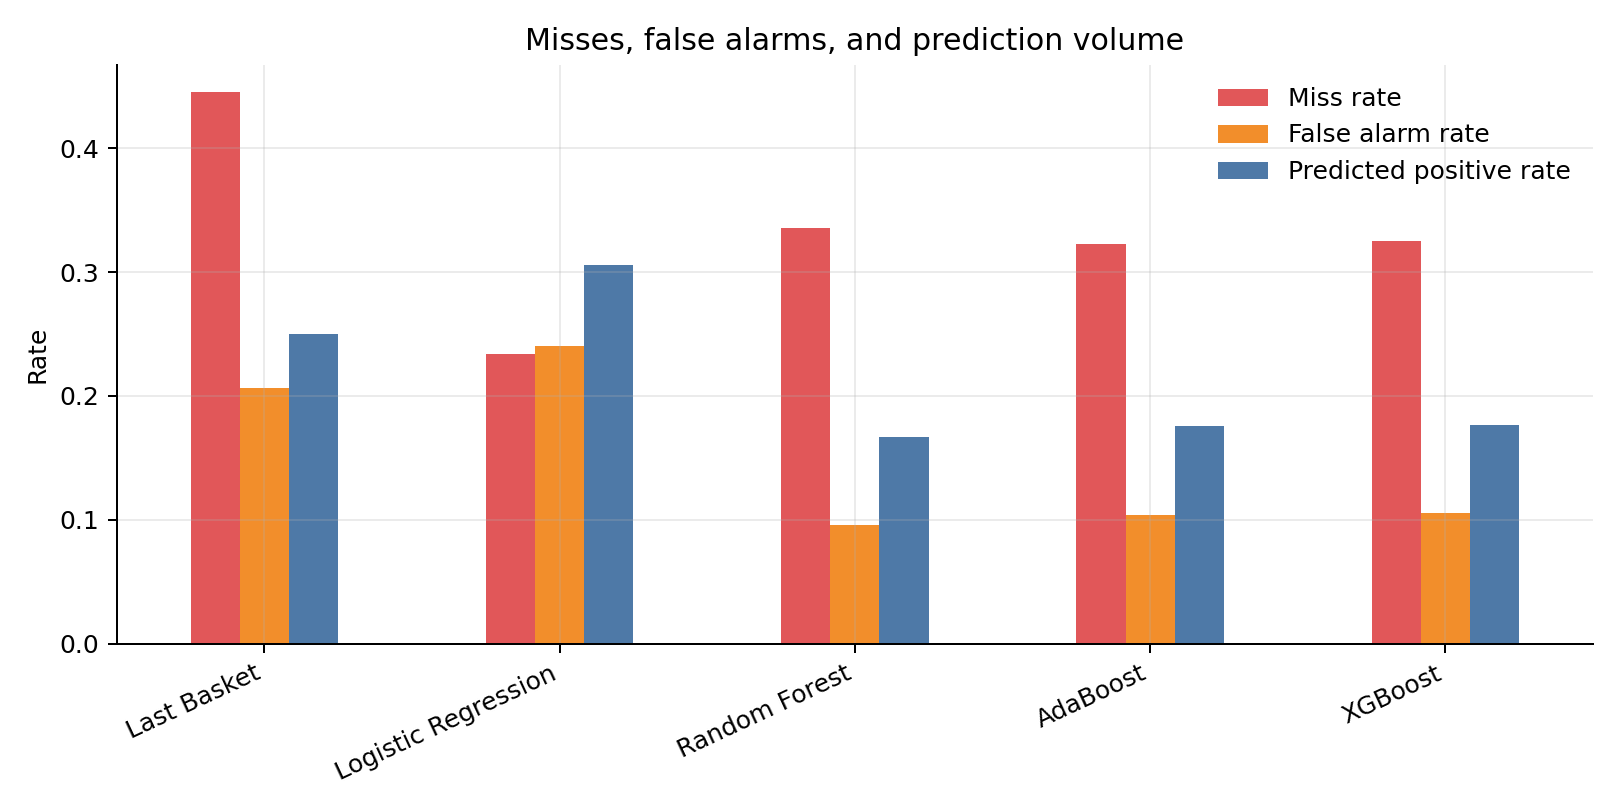
\includegraphics[width=\linewidth]{02_error_rates.png}
\subcaption{Miss, false-alarm, and predicted-positive rates.}
\label{fig:errorrates}
\end{minipage}\hfill
\begin{minipage}[t]{0.48\textwidth}
\centering
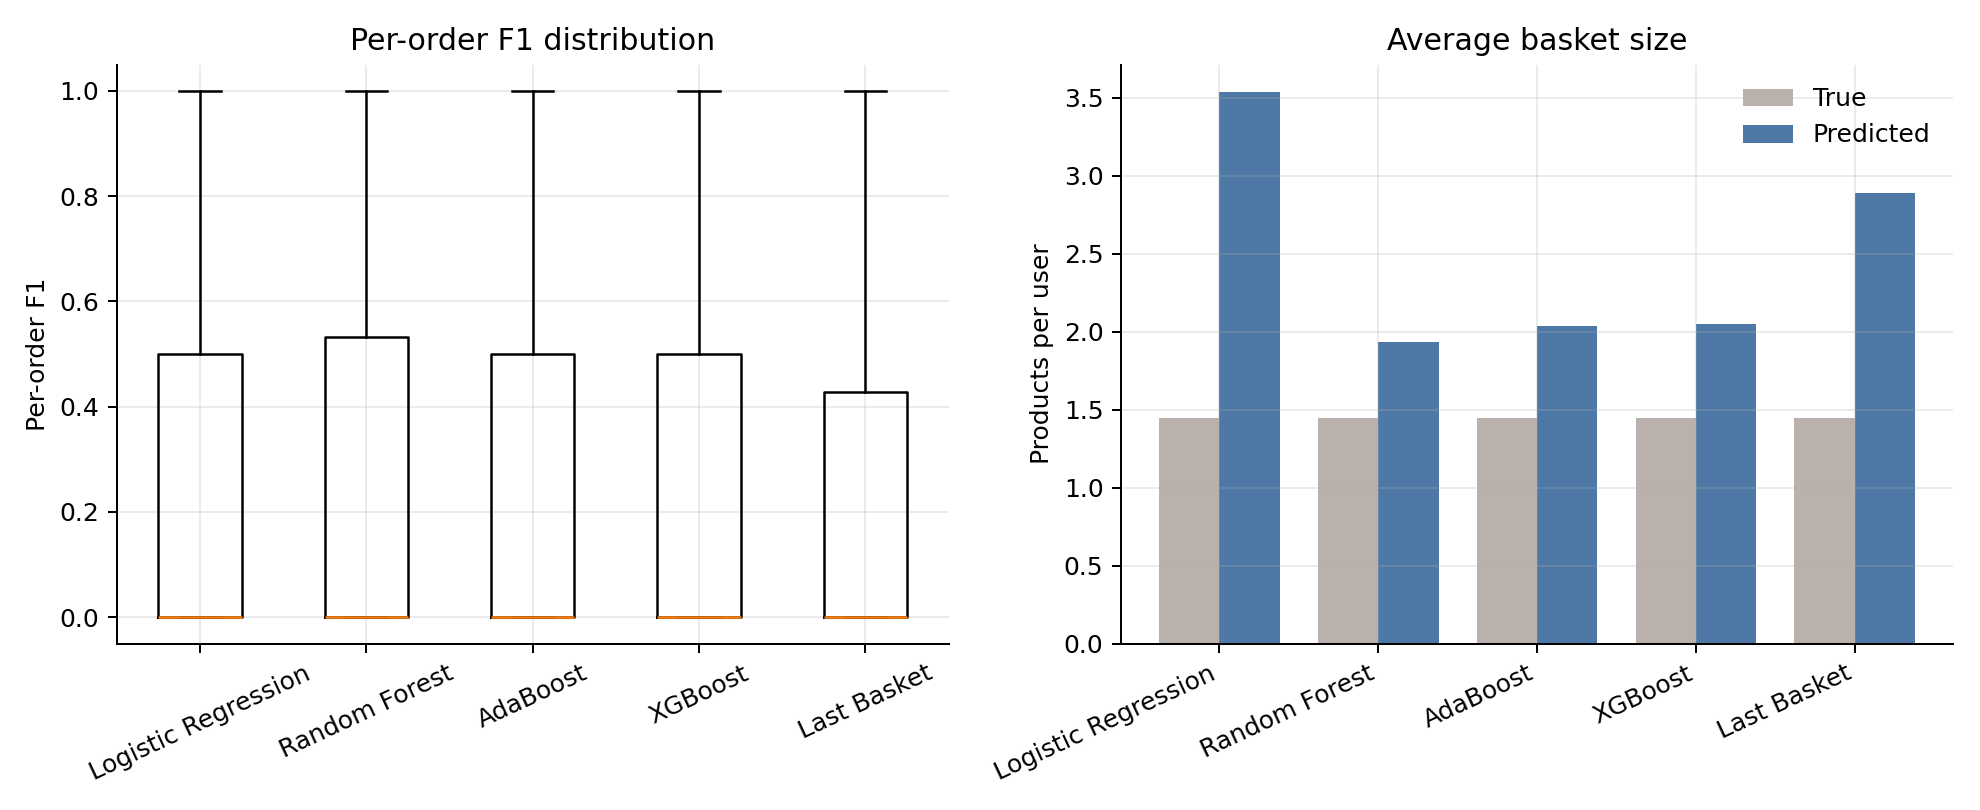
\includegraphics[width=\linewidth]{04_basket_metrics.png}
\subcaption{Per-order F1 distribution and average predicted basket size.}
\label{fig:basket}
\end{minipage}
\caption{Error and basket-level views of the row-vs-order F1 reversal. \textbf{(a)} Logistic regression is recall-heavy with the highest predicted-positive rate; random forest is the most conservative. \textbf{(b)} Logistic regression's per-order F1 advantage comes from predicting substantially larger baskets (3.54 products) than the true mean (1.45) and than random forest (1.93).}
\label{fig:rowvsorder}
\end{figure*}

\subsection{Basket-Level Behavior}

The basket-level analysis shows why per-order F1 differs from row-level F1. The true average reordered basket size is 1.45 products. Random forest predicts 1.93 products per user on average, while logistic regression predicts 3.54. This larger basket raises recall and per-order F1, but with a high false-positive cost. Logistic regression has a basket-size mean absolute error of 2.32, compared with 0.92 for random forest.

\subsection{Effect Sizes and Statistical Tests}

Table~\ref{tab:effects} reports raw effect sizes relative to random forest. All tree-model versus baseline comparisons reach statistical significance under McNemar's test ($p < 10^{-3}$) after Bonferroni correction. However, the user-bootstrap 95\% confidence interval for the RF--AdaBoost per-order F1 difference is $[-0.0014, +0.0079]$, which contains zero. Even when paired tests are statistically significant due to large $N$, absolute differences below $\sim$0.005 F1 should be interpreted cautiously as practically small.

\begin{table}[t]
\centering
\caption{Random forest effect sizes versus alternative models. Positive values mean random forest is higher.}
\label{tab:effects}
\scriptsize
\begin{tabular}{lrrrr}
\toprule
Comparison & Row F1 & Order F1 & ROC & PR \\
\midrule
RF -- AdaBoost & +0.0056 & +0.0011 & +0.0053 & +0.0107 \\
RF -- XGBoost & +0.0099 & +0.0035 & +0.0027 & -0.0009 \\
RF -- LogReg & +0.1240 & -0.0055 & +0.0645 & +0.1138 \\
RF -- Last Basket & +0.1985 & +0.0357 & +0.1501 & +0.3357 \\
\bottomrule
\end{tabular}
\end{table}

\subsection{Model Disagreement and Error Overlap}

The model-disagreement analysis addresses the project objective directly: where do models fail differently? Figure~\ref{fig:overlap} shows two patterns. First, the tree ensembles are similar to each other, especially random forest and XGBoost, which have only a 4.1\% prediction disagreement rate and a 0.724 error-overlap Jaccard. Second, logistic regression disagrees more with the trees because it predicts positives much more aggressively. This suggests that an ensemble could benefit more from combining a tree model with logistic regression than from combining the three tree ensembles alone.

\begin{figure*}[t]
\centering
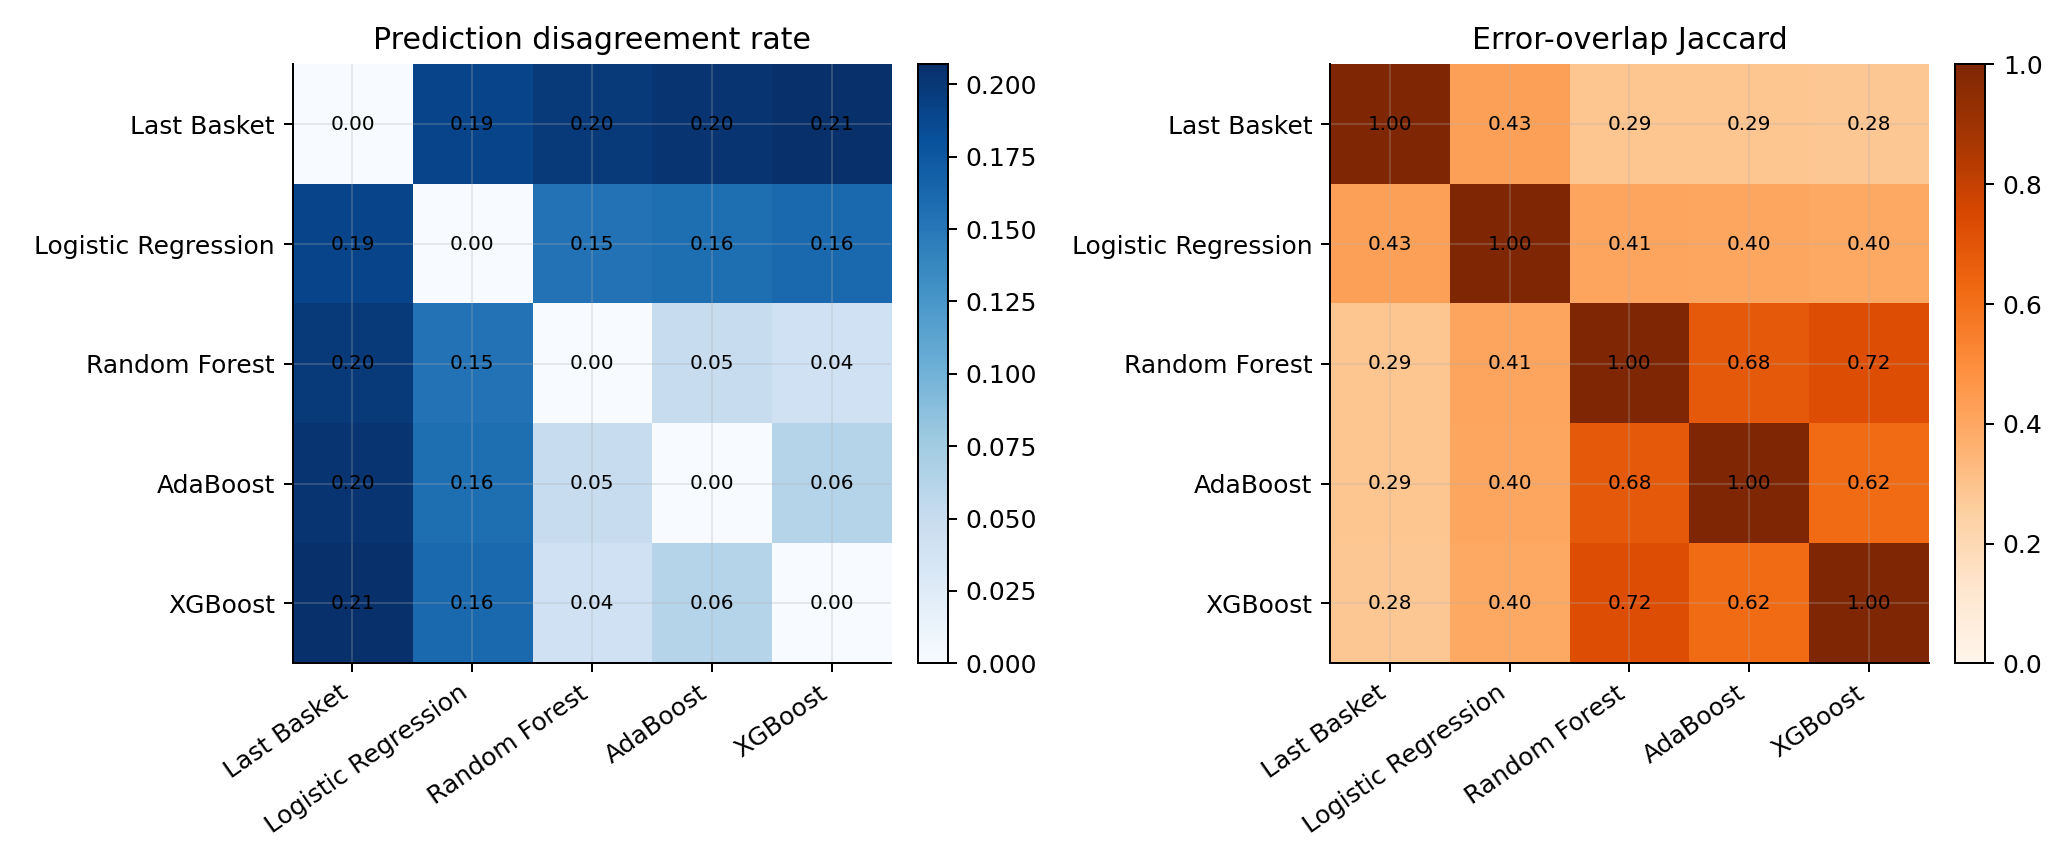
\includegraphics[width=0.9\textwidth]{05_model_disagreement_overlap.png}
\caption{Pairwise prediction disagreement and error-overlap Jaccard. Tree ensembles share many errors; logistic regression has a different error profile driven by high recall and larger baskets.}
\label{fig:overlap}
\end{figure*}

\section{Subgroup and Stratified Error Analysis}
\label{sec:strat}

The global metrics from the previous section obscure cohort-level behavioral differences. We disaggregate the controlled test set across three orthogonal axes --- product reorder rate, user activity, and aisle purchase variance --- and recompute precision, recall, and F1 within each cohort. The product axis buckets candidate rows by each product's prior-only global reorder rate (high $\geq 0.60$, mid $0.20$--$0.60$, occasional $< 0.20$); the user axis buckets users by total prior orders (cold-start $<5$, regular $5$--$29$, power user $\geq 30$); the aisle axis uses the EDA's standard-deviation-of-product-reorder-rate measure (top-20 aisles by std as ``high variance,'' bottom-20 as ``low variance,'' filtered to aisles with at least five products). Table~\ref{tab:strat} summarizes the within-cohort F1 leaders.

\begin{table*}[t]
\centering
\footnotesize
\setlength{\tabcolsep}{5pt}
\renewcommand{\arraystretch}{1.05}
\caption{Stratified Performance Analysis. Within-cohort F1 leader (and runner-up) plus the dominant error mode for the leader on each cohort. Numbers are computed on the same controlled 75{,}000-row test set as Table~\ref{tab:metrics}. ``FA'' is false-alarm rate; ``Miss'' is FN/positives.}
\label{tab:strat}
\begin{tabular}{l l r r l c c}
\toprule
\textbf{Axis} & \textbf{Cohort} & \textbf{$n$} & \textbf{Pos.\ rate} & \textbf{Leader (F1) / Runner-up} & \textbf{Failure mode} & \textbf{Rate} \\
\midrule
Product reorder rate & High ($\geq 60\%$)     & 39{,}793 & 0.169 & RF (0.605) / AdaBoost (0.601)     & FA-lean       & 0.148 \\
Product reorder rate & Mid ($20$--$60\%$)     & 33{,}719 & 0.078 & RF (0.454) / XGBoost (0.453)      & Miss-dominant & 0.547 \\
Product reorder rate & Occasional ($<20\%$)   &  1{,}488 & 0.011 & LogReg (0.167) / XGBoost (0.111)  & Miss-dominant & 0.875 \\
\midrule
User activity        & Cold-start ($<5$)      &  3{,}531 & 0.135 & AdaBoost (0.524) / RF (0.520)     & Miss-dominant & 0.371 \\
User activity        & Regular ($5$--$29$)    & 37{,}746 & 0.128 & RF (0.562) / XGBoost (0.554)      & Miss-lean     & 0.344 \\
User activity        & Power user ($\geq 30$) & 33{,}723 & 0.121 & AdaBoost (0.582) / RF (0.582)     & Miss-dominant & 0.308 \\
\midrule
Aisle variance       & High variance (top-20) &  6{,}520 & 0.159 & RF (0.647) / AdaBoost (0.646)     & FA-lean       & 0.114 \\
Aisle variance       & Low variance (bot.-20) &  5{,}969 & 0.097 & RF (0.552) / XGBoost (0.546)      & Miss-dominant & 0.390 \\
\bottomrule
\end{tabular}
\end{table*}

Three findings reshape the headline ranking. First, no single model wins all eight cohorts: random forest leads five of eight, AdaBoost matches or wins on the cold-start and power-user cohorts, and logistic regression is the only model with non-zero F1 on the occasional-product cohort (0.167; random forest predicts no positives). The occasional-product cohort contains only 1{,}488 rows at a 1.1\% positive rate, so its absolute F1 numbers warrant statistical caution. This matches the disagreement profile in Figure~\ref{fig:overlap}: tree ensembles agree on most rows but diverge from logistic regression on the long tail of low-reorder products. Second, even on the low-variance aisle cohort --- where the last-basket heuristic is closest to optimal --- random forest's F1 of 0.552 is 0.24 absolute above last-basket (0.313), so machine learning continues to add measurable value even where staple cadence is most predictable. The advantage shrinks on the high-variance cohort to 0.21, but does not vanish. Third, the dominant failure mode varies by cohort in interpretable ways. High-reorder and high-variance cohorts tend toward false alarms because the model over-predicts when the prior is high. In contrast, mid-tier products, occasional products, and the user-activity cohorts are dominated by misses, with recall becoming the limiting factor. The implication is that operational threshold tuning should not be global; cohort-specific thresholds are likely to recover meaningful F1 on the miss-dominant slices.

A complementary none-user breakdown is consistent with this picture: random forest's F1 collapses from 0.61 on regular users to 0.04 on none-users because every positive prediction in a none-user basket is a forced false alarm; random forest's low overall false-alarm rate (0.026 on none-users vs.\ 0.205 for logistic regression) keeps that collapse the smallest among the ML models.

\subsection{Behavioral Error Tags}

Behavioral tags are programmatically assigned labels for common error modes. Each tag is a Boolean predicate over the row's error type and feature values. For reporting, each row is assigned its first matching tag (in the order below) for reportability.
\begin{itemize}
\setlength{\itemsep}{0pt}
\setlength{\parskip}{0pt}
\setlength{\topsep}{2pt}
\item \textbf{Stockpile (FP)}: $\text{up\_purchase\_count} \geq 3$, $\text{up\_orders\_since\_last} \leq 1$, and $\text{target\_days\_since\_prior} \leq 7$ --- model repeats a frequently bought item that the user just bought and has not had time to deplete.
\item \textbf{Broken-streak (FP)}: $\text{up\_streak} \geq 2$ --- model expects a multi-order purchase streak to continue, but it does not.
\item \textbf{Recipe / novelty (FP)}: $\text{up\_purchase\_count} = 1$ and $\text{prod\_reorder\_ratio} < 0.45$ --- model repeats a one-time, low-reorder item.
\item \textbf{Sleeper-staple (FN)}: $\text{up\_purchase\_count} \geq 3$, $\text{up\_orders\_since\_last} \geq 3$, and $\text{prod\_reorder\_ratio} \geq 0.45$ --- model misses a popular staple after a multi-order absence.
\item \textbf{New-habit (FN)}: $\text{up\_purchase\_count\_n5} \geq 2$ and $\text{up\_orders\_since\_last\_n5} \leq 1$ --- model misses a recently emerged habit.
\item \textbf{Basket-size inflation (large)}: $\text{pred\_basket} - \text{true\_basket} \geq \max(3,\, \lceil 0.5 \cdot \text{true\_basket}\rceil)$.
\item \textbf{None-collapse}: $\text{true\_basket} = 0$ and $\text{pred\_basket} = 0$ (correct empty-basket behavior on none-users; flagged for behavioral analysis rather than as an error).
\end{itemize}

Quantitatively, basket-size-inflation tags account for $36.7\%$ of logistic regression's flagged rows versus $13.5\%$ of XGBoost's and $11.7\%$ of random forest's, a $\sim 2.7\times$ gap that mechanically explains the per-order F1 reversal in Table~\ref{tab:metrics}: logistic regression recovers more reorders per basket precisely because it predicts substantially larger baskets, with the false-alarm cost concentrated in basket-size-inflation tags rather than in recipe or stockpile errors.

\begin{figure}[t]
\centering
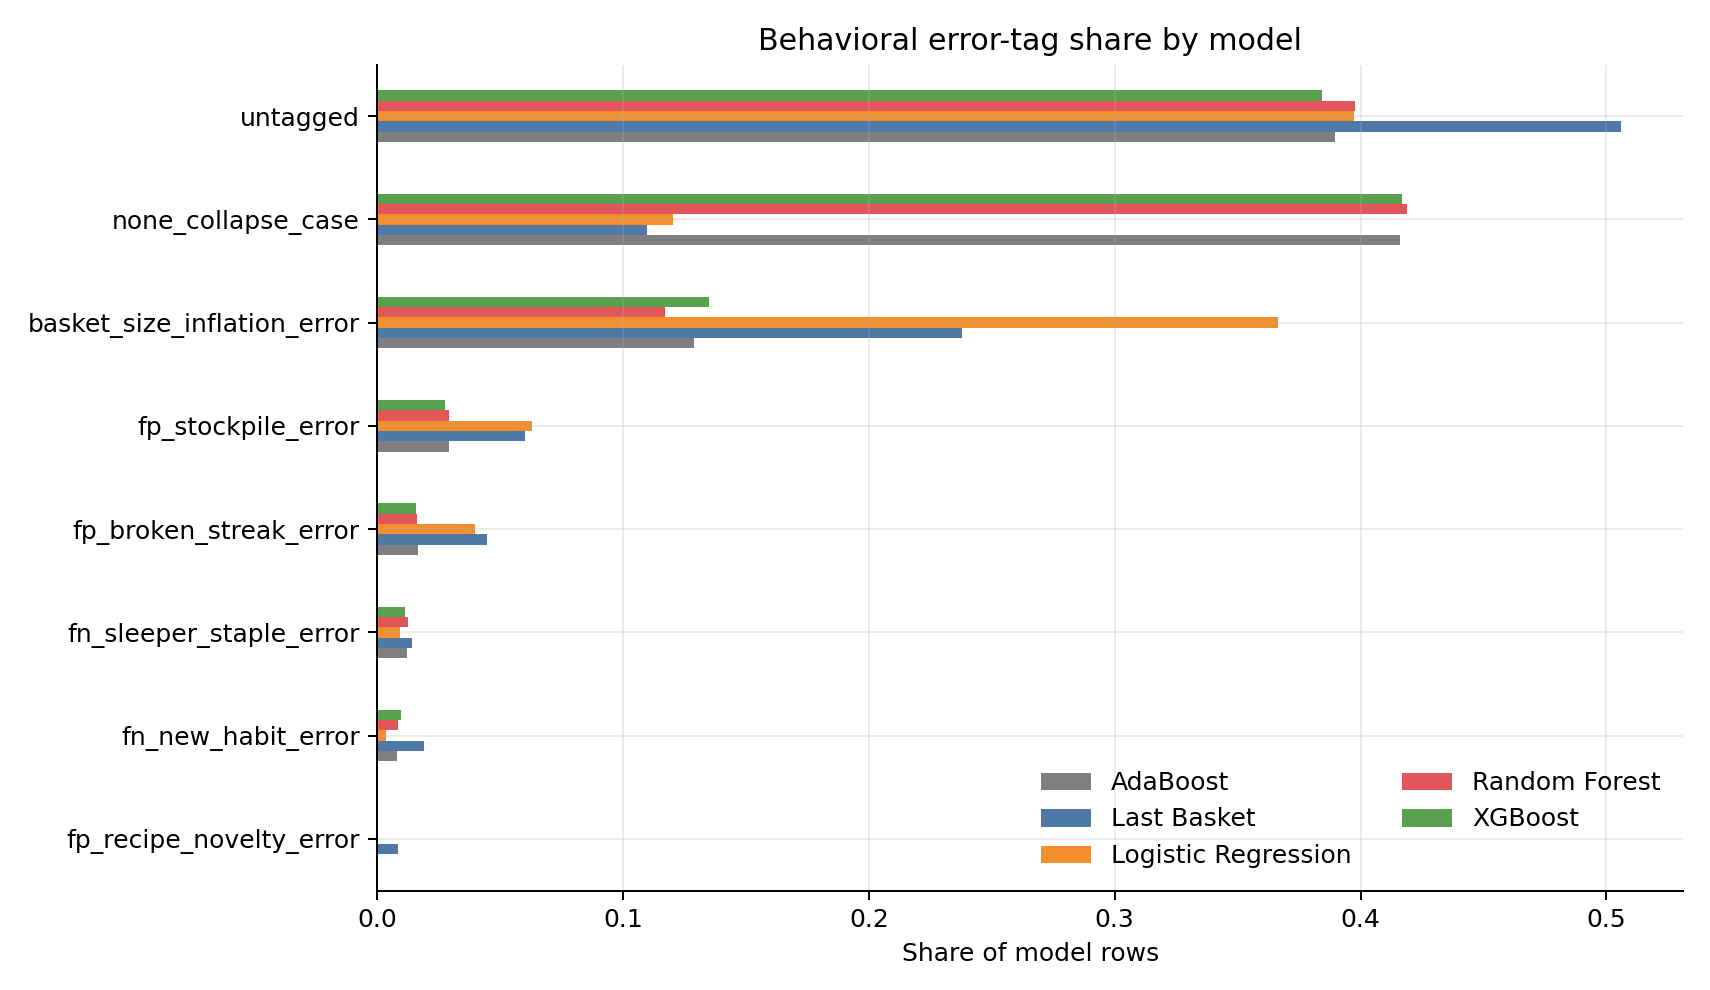
\includegraphics[width=\columnwidth]{07_behavioral_error_tags.png}
\caption{Behavioral error tag shares. Basket-size inflation is especially common for logistic regression and the last-basket baseline.}
\label{fig:tags}
\end{figure}

\section{Feature Importance}

Because all models were trained on the same feature set, built-in importance rankings can be compared meaningfully. The strongest tree-model features are dominated by recency and user--product behavior: target days since prior order, user--product purchase counts in the last five orders, orders since last purchase, day-of-week purchase counts, and reorder-rate summaries. This matches the prior competition observation that recency-windowed user--item features are highly predictive \citep{onodera2017instacart}.

The four built-in importance scores in Figure~\ref{fig:importance} are computed by fundamentally different mechanisms --- standardized coefficients for logistic regression, mean-decrease-in-impurity for random forest and AdaBoost, and split-gain for XGBoost. Consequently, the x-axis scales are model-specific, and the bars represent intra-model rankings rather than directly comparable cross-model magnitudes. The Jaccard overlap analysis in Table~\ref{tab:featureoverlap} sidesteps this scaling issue by comparing only the set membership of each model's top-10 features.

\begin{figure*}[t]
\centering
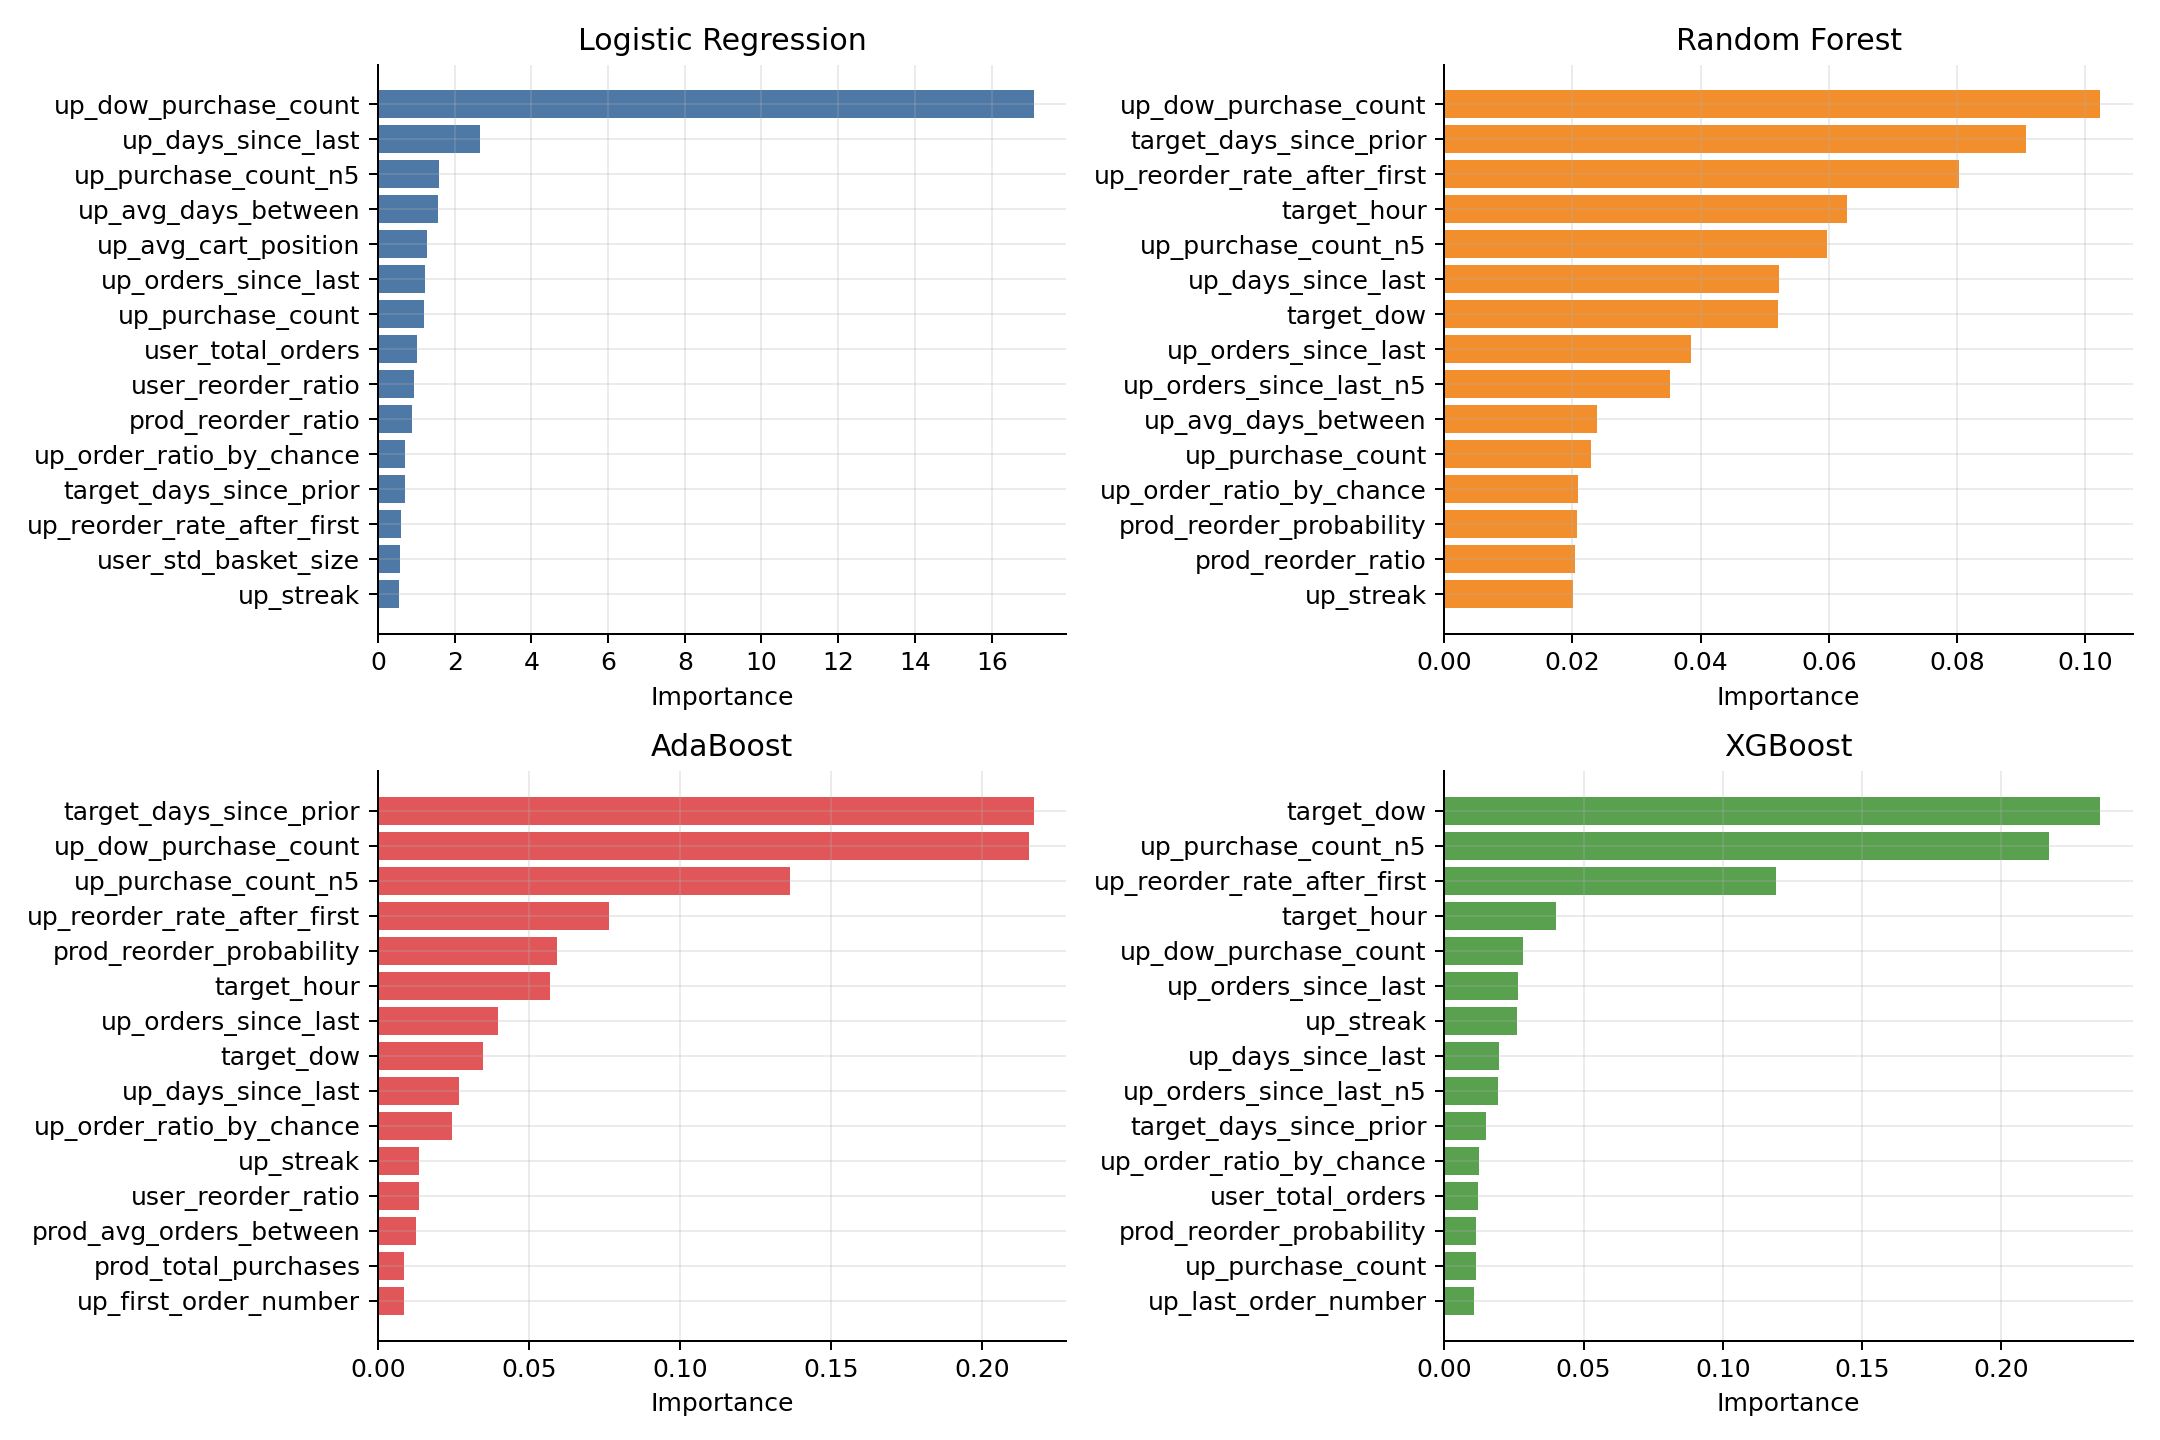
\includegraphics[width=0.9\textwidth]{08_feature_importance_top15.png}
\caption{Top built-in feature importances for the four ML models. Tree ensembles emphasize recency and user--product interaction features; logistic regression's ranking is less aligned with the tree models.}
\label{fig:importance}
\end{figure*}

\begin{table}[t]
\centering
\caption{Jaccard overlap of each model's top-10 built-in importance features.}
\label{tab:featureoverlap}
\scriptsize
\begin{tabular}{lrrrr}
\toprule
Model & LogReg & RF & Ada & XGB \\
\midrule
LogReg & 1.000 & 0.333 & 0.250 & 0.250 \\
RF & 0.333 & 1.000 & 0.667 & \textbf{0.818} \\
Ada & 0.250 & 0.667 & 1.000 & 0.667 \\
XGB & 0.250 & \textbf{0.818} & 0.667 & 1.000 \\
\bottomrule
\end{tabular}
\end{table}

Table~\ref{tab:featureoverlap} reinforces the model-disagreement result. Random forest and XGBoost have the most similar top-10 feature sets, while logistic regression overlaps only weakly with the boosted and bagged trees. Thus, the shared-input design reveals a substantive modeling difference: the tree models use similar nonlinear recency signals, whereas the linear model reaches its high recall through a different weighting of the same feature space.

\section{Discussion}

The main controlled result is that random forest is the strongest row-level classifier. It has the best F1 and ROC-AUC, the lowest false-alarm rate, and the best basket-size calibration. XGBoost remains competitive and has the best PR-AUC, making it the strongest scalable boosted-tree candidate. AdaBoost is close to random forest but slightly worse on row F1 and false alarms.

The most important interpretive result is that the headline model changes under per-order F1. Logistic regression wins per-order F1 despite weaker row-level precision because it predicts much larger baskets and therefore captures more true reorders. A likely explanation is its inductive bias: a linear, additive scoring rule with a single threshold has less ability to isolate the nonlinear recency-frequency-product interactions that the tree ensembles split on natively, which may cause it to assign moderate scores across more candidate rows and over-predict the basket. The tree models, by contrast, can carve out small recency-times-frequency pockets of high reorder probability and threshold tightly inside them, which produces smaller, more precise predicted baskets. This is not a contradiction; it is a metric-dependent tradeoff. For an operational recommender where over-recommending products is costly, random forest would be preferable. For a setting where missing a reorder is much worse than showing extra candidates, logistic regression may be defensible. Concretely: in a screen-real-estate-constrained surface (a four-tile mobile carousel), random forest's smaller, sharper basket dominates because every false alarm displaces a useful suggestion; in a recall-dominant channel (a weekly reminder email or a long scrollable shopping list), logistic regression's larger, lower-precision basket can recover more reorder volume per impression, with the false-alarm cost diluted by abundant surface area.

The last-basket baseline is strong enough to serve as a meaningful sanity check but is clearly beaten by every ML model on row-level F1, ROC-AUC, PR-AUC, and per-order F1. This confirms that engineered user--product and timing features add signal beyond a pure recency heuristic.

A practical implication of the model-disagreement pattern (visualized in the error-overlap matrix of Figure~\ref{fig:overlap}) is that a stacked or learned ensemble that explicitly exploits the gap between logistic regression and the tree ensembles is more promising than ensembling the three tree models among themselves.

\section{Limitations and Future Work}

The feature-importance analysis in this study uses each model's built-in importance scores. A natural extension is to corroborate these rankings with model-agnostic permutation importance and with drop-one and group-ablation refits, which would isolate the marginal contribution of each feature group (user, product, user~$\times$~product, datetime) under each algorithm and provide a stronger basis for the cross-model importance comparison in Table~\ref{tab:featureoverlap}.

The final controlled evaluation reports each model on a common 75{,}000-row, 6{,}484-user sample drawn from the held-out test set, which is the fair comparison given the shared training and test caps and the inclusion of the last-basket baseline. The next step is to scale the same evaluation pipeline to the full 206{,}000-user candidate table and to verify that the metric ordering and the behavioral error-tag distributions are stable.

Finally, the model-disagreement analysis in Figure~\ref{fig:overlap} suggests a concrete two-stage stacked ensemble: use logistic regression as a high-recall candidate-generator that emits an over-complete shortlist of likely reorders (recovering the occasional-product cohort where tree ensembles in Table~\ref{tab:strat} predict no positives at all), then use XGBoost as a high-precision re-ranker that trims the shortlist to a calibrated basket. The fact that LogReg and XGBoost share only $25\%$ of their top-10 features (Table~\ref{tab:featureoverlap}) is what makes the stack non-trivial: the two stages fail in different cohorts, so each compensates for the other's blind spot rather than amplifying a shared bias.

\section{Conclusion}

This study demonstrates that model ranking for Instacart reorder prediction is highly sensitive to the chosen evaluation metric. Random forest excels at row-level classification and precision, while logistic regression dominates per-order F1 by predicting systematically larger baskets. The comparative error analysis reveals that while tree ensembles share redundant error modes, linear models fail differently --- highlighting that operational recommender design must be guided by the asymmetric costs of false alarms versus missed staples, rather than a single classification metric.

\section*{Appendix: Final Hyperparameters}

To ensure reproducibility, the final tuned hyperparameters are: \textbf{Logistic Regression}: \texttt{C=100}, L2 penalty, balanced class weight. \textbf{Random Forest}: 500 estimators, \texttt{max\_depth=20}, \texttt{min\_samples\_split=5}, \texttt{min\_samples\_leaf=1}, \texttt{max\_features=sqrt}, balanced class weight. \textbf{AdaBoost}: 100 estimators, \texttt{learning\_rate=1.0}, depth-3 \texttt{DecisionTreeClassifier} base estimator. \textbf{XGBoost}: \texttt{learning\_rate=0.0307}, \texttt{max\_depth=10}, \texttt{min\_child\_weight=8}, \texttt{subsample=0.880}, \texttt{colsample\_bytree=0.747}, \texttt{gamma=0.078}, 1999 estimators, \texttt{scale\_pos\_weight=6.88}.

\balance
\setlength{\bibsep}{0.5pt plus 0.1ex}
{\scriptsize
\bibliographystyle{plainnat}
\bibliography{references}}

\end{document}
